\documentclass[12pt]{article}
	\usepackage{graphicx,amsmath}
	\usepackage[round]{natbib}
	\usepackage[margin=3cm]{geometry}
	\linespread{1.3}
	\bibliographystyle{plainnat}
	\title{
		Group \#07 \\
		Bridge-00 \\
		18g, 1700N \\[1cm]
		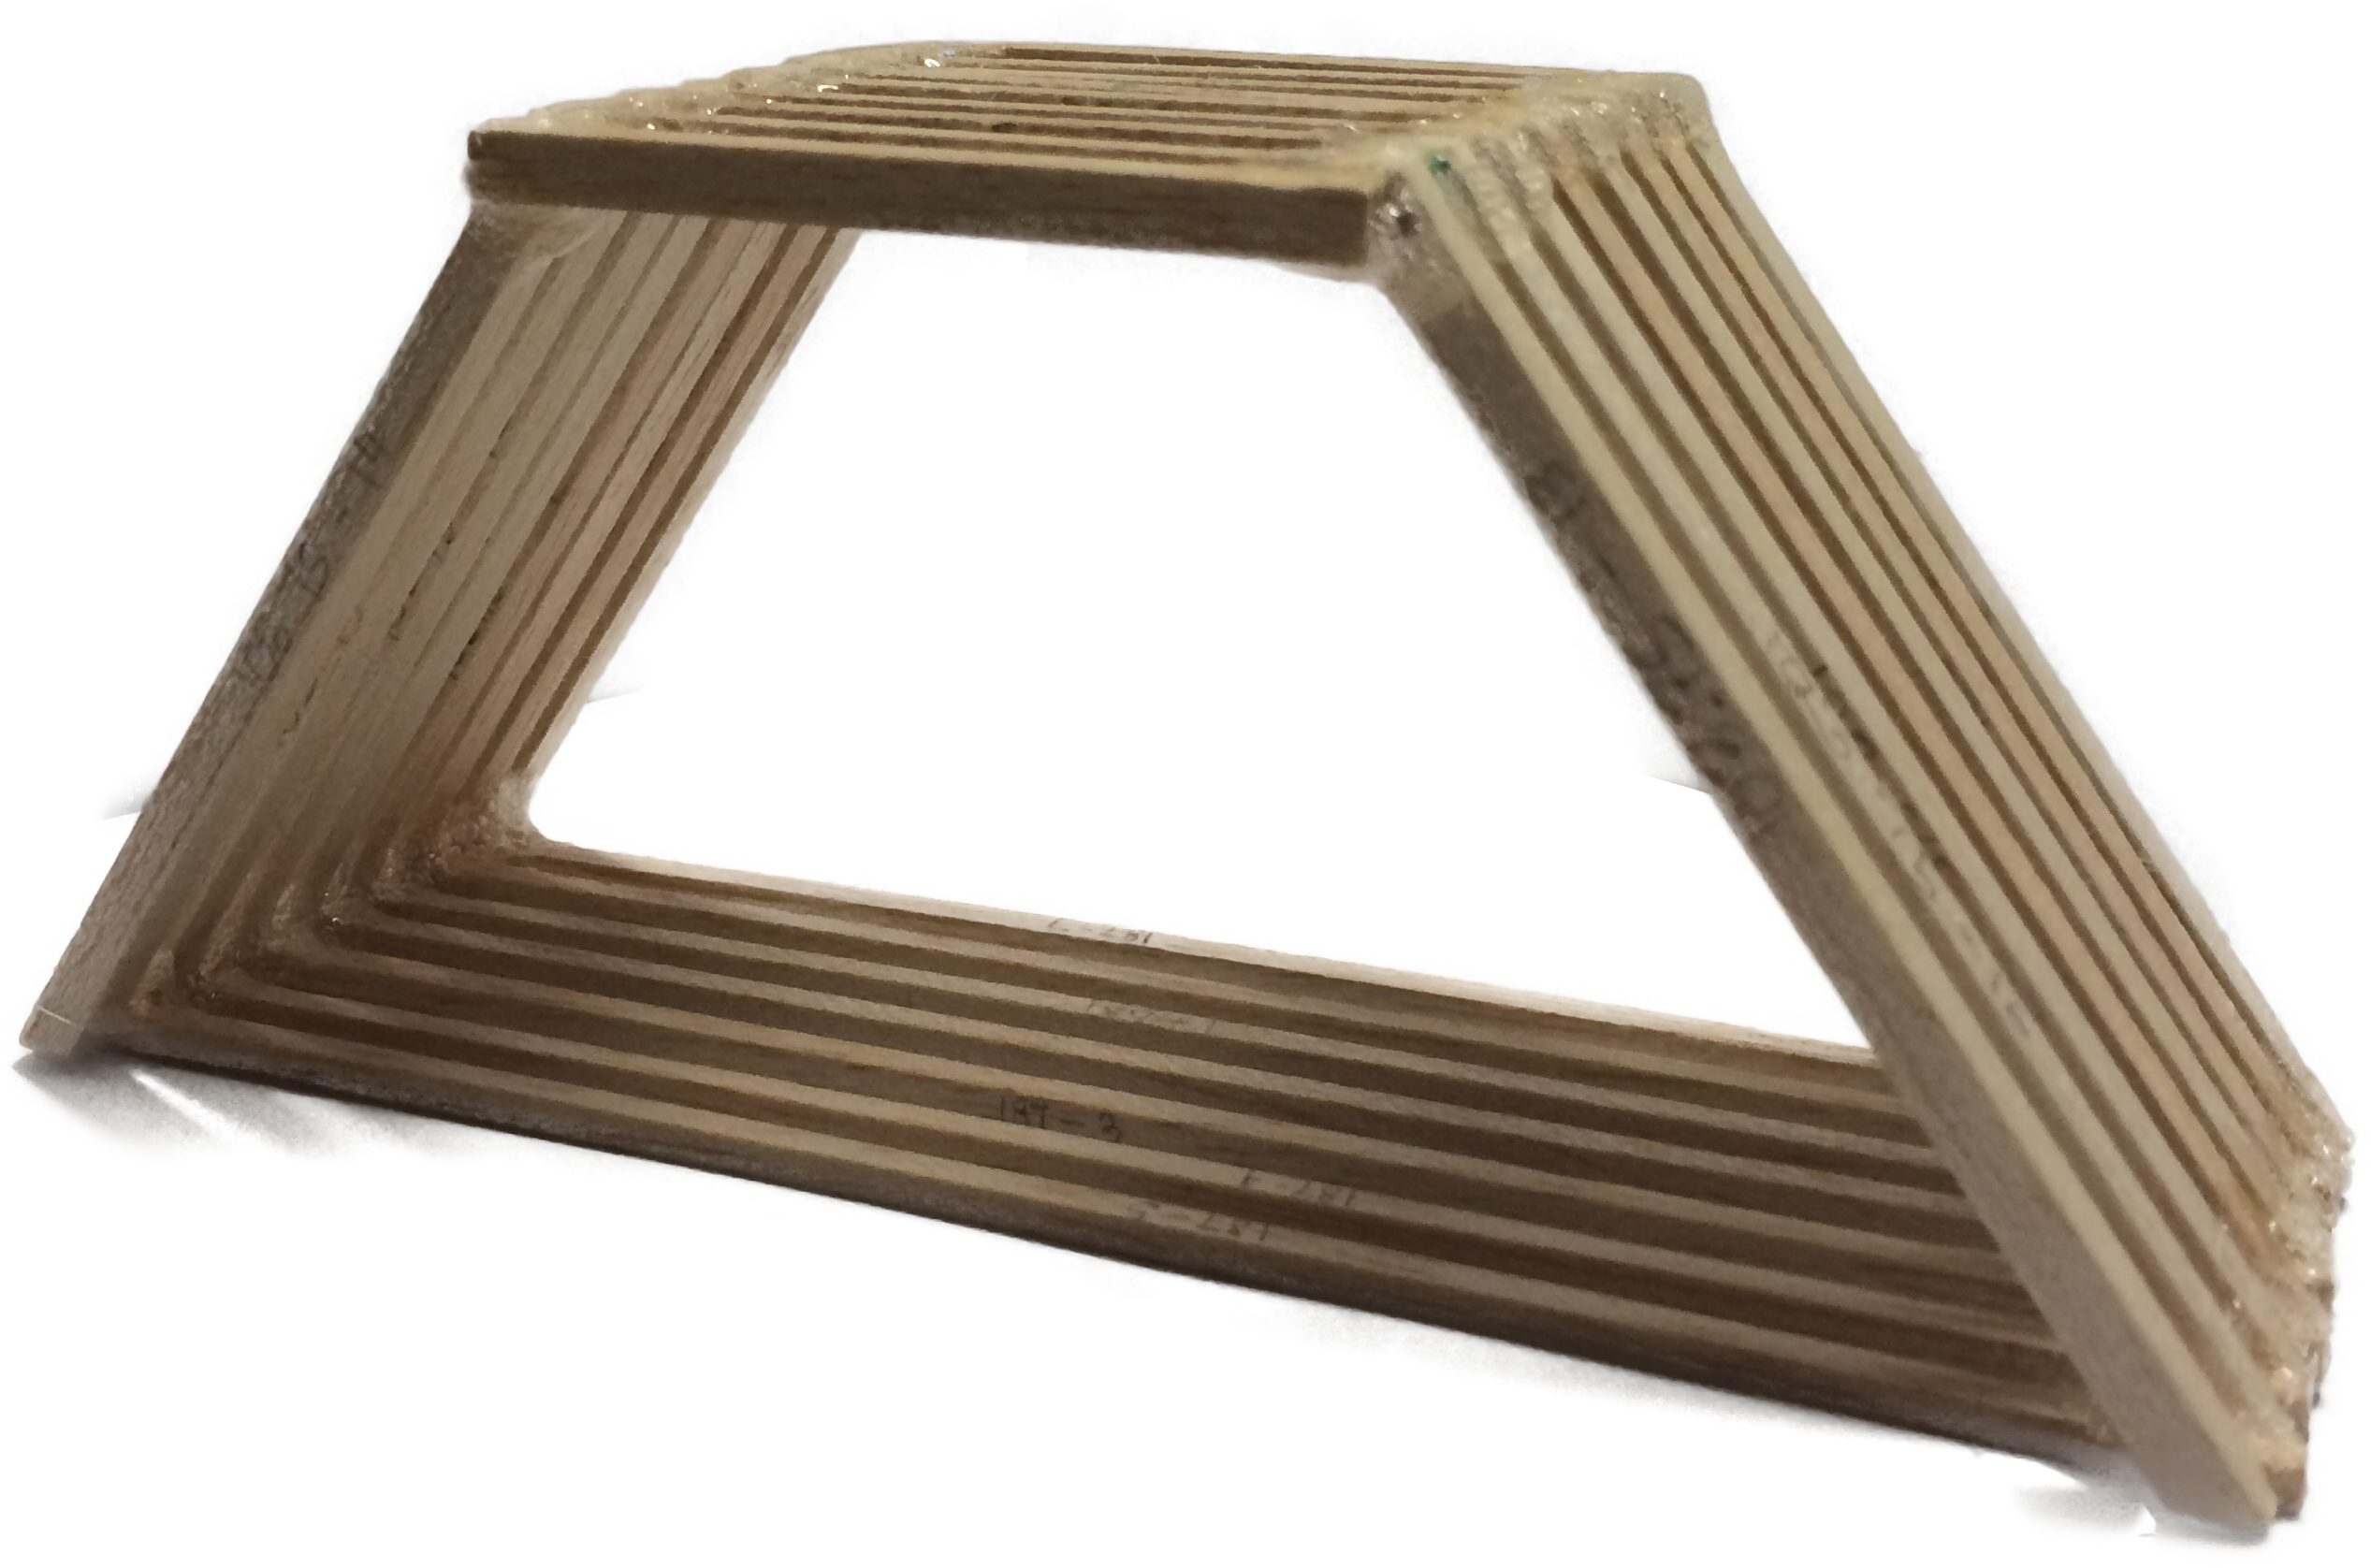
\includegraphics[width=0.7\textwidth]{photo}
	}
	\author{
		Alex Miles \\ u5568175 \\ 16.7\%
		\and Arlene Mendoza \\ u5589650 \\ 16.7\%
		\and Itsuki Nishida \\ u5578430 \\ 16.7\%
		\and Paul Apelt \\ u5568225 \\ 16.7\%
		\and Stephen Lonergan \\ u5349877 \\ 16.7\%
		\and Thomas Hale \\ u5568225 \\ 16.7\%
	}
\begin{document}
	\maketitle
	\thispagestyle{empty}
	\setcounter{page}{0}
	\section{Design}
		% design assumptions and methods
		\subsection{Assumptions}
		During the design process, the following assumptions have been made \citep[p.~264]{tbook}:
		\begin{enumerate}
			\item All loadings are applied at the joint,
			\item Weight of the members neglected,
			\item Joints are smooth (friction-less) pins,
			\item Each member has no more than two joints.
		\end{enumerate}
		% TODO: why trapezium
		% other designs considered
		% photo of a prototype
		Final bridge design can be seen in Figures \ref{dim} and \ref{proj}.
		\begin{figure}[h!]
			\centering
			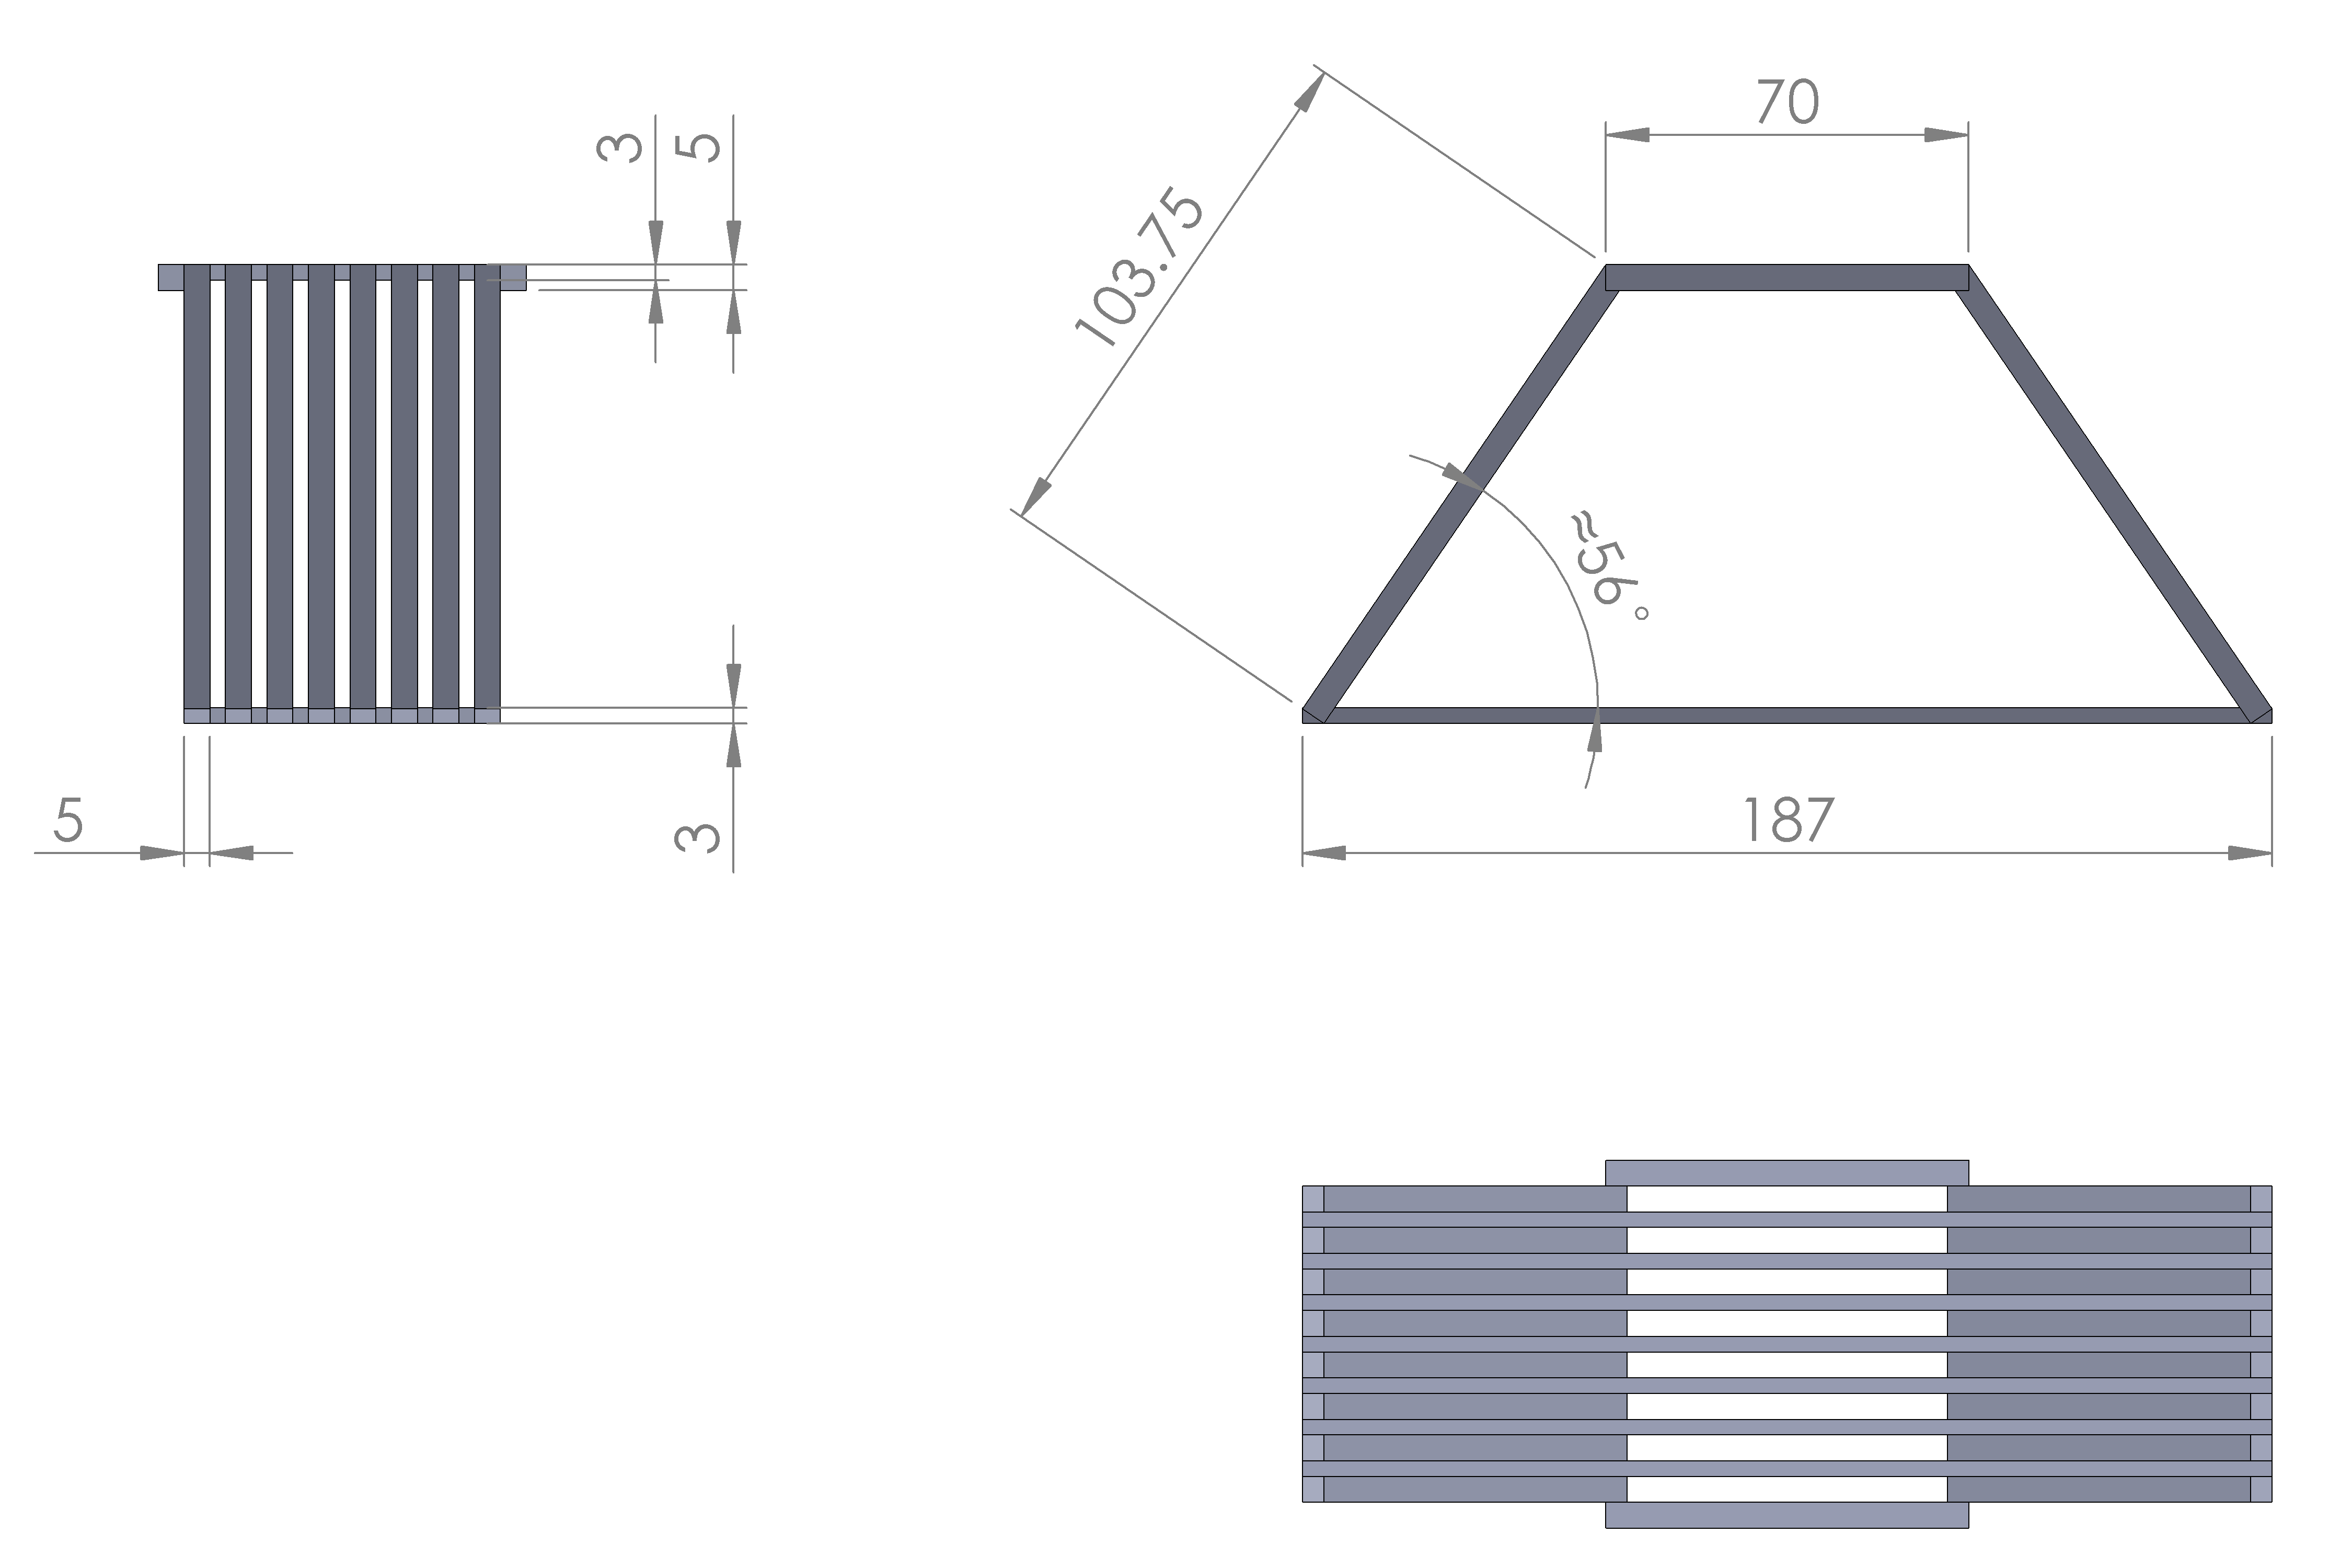
\includegraphics[width=\textwidth]{dim}
			\caption{Dimensioned drawing.}
			\label{dim}
		\end{figure}
		\begin{figure}[h!]
			\centering
			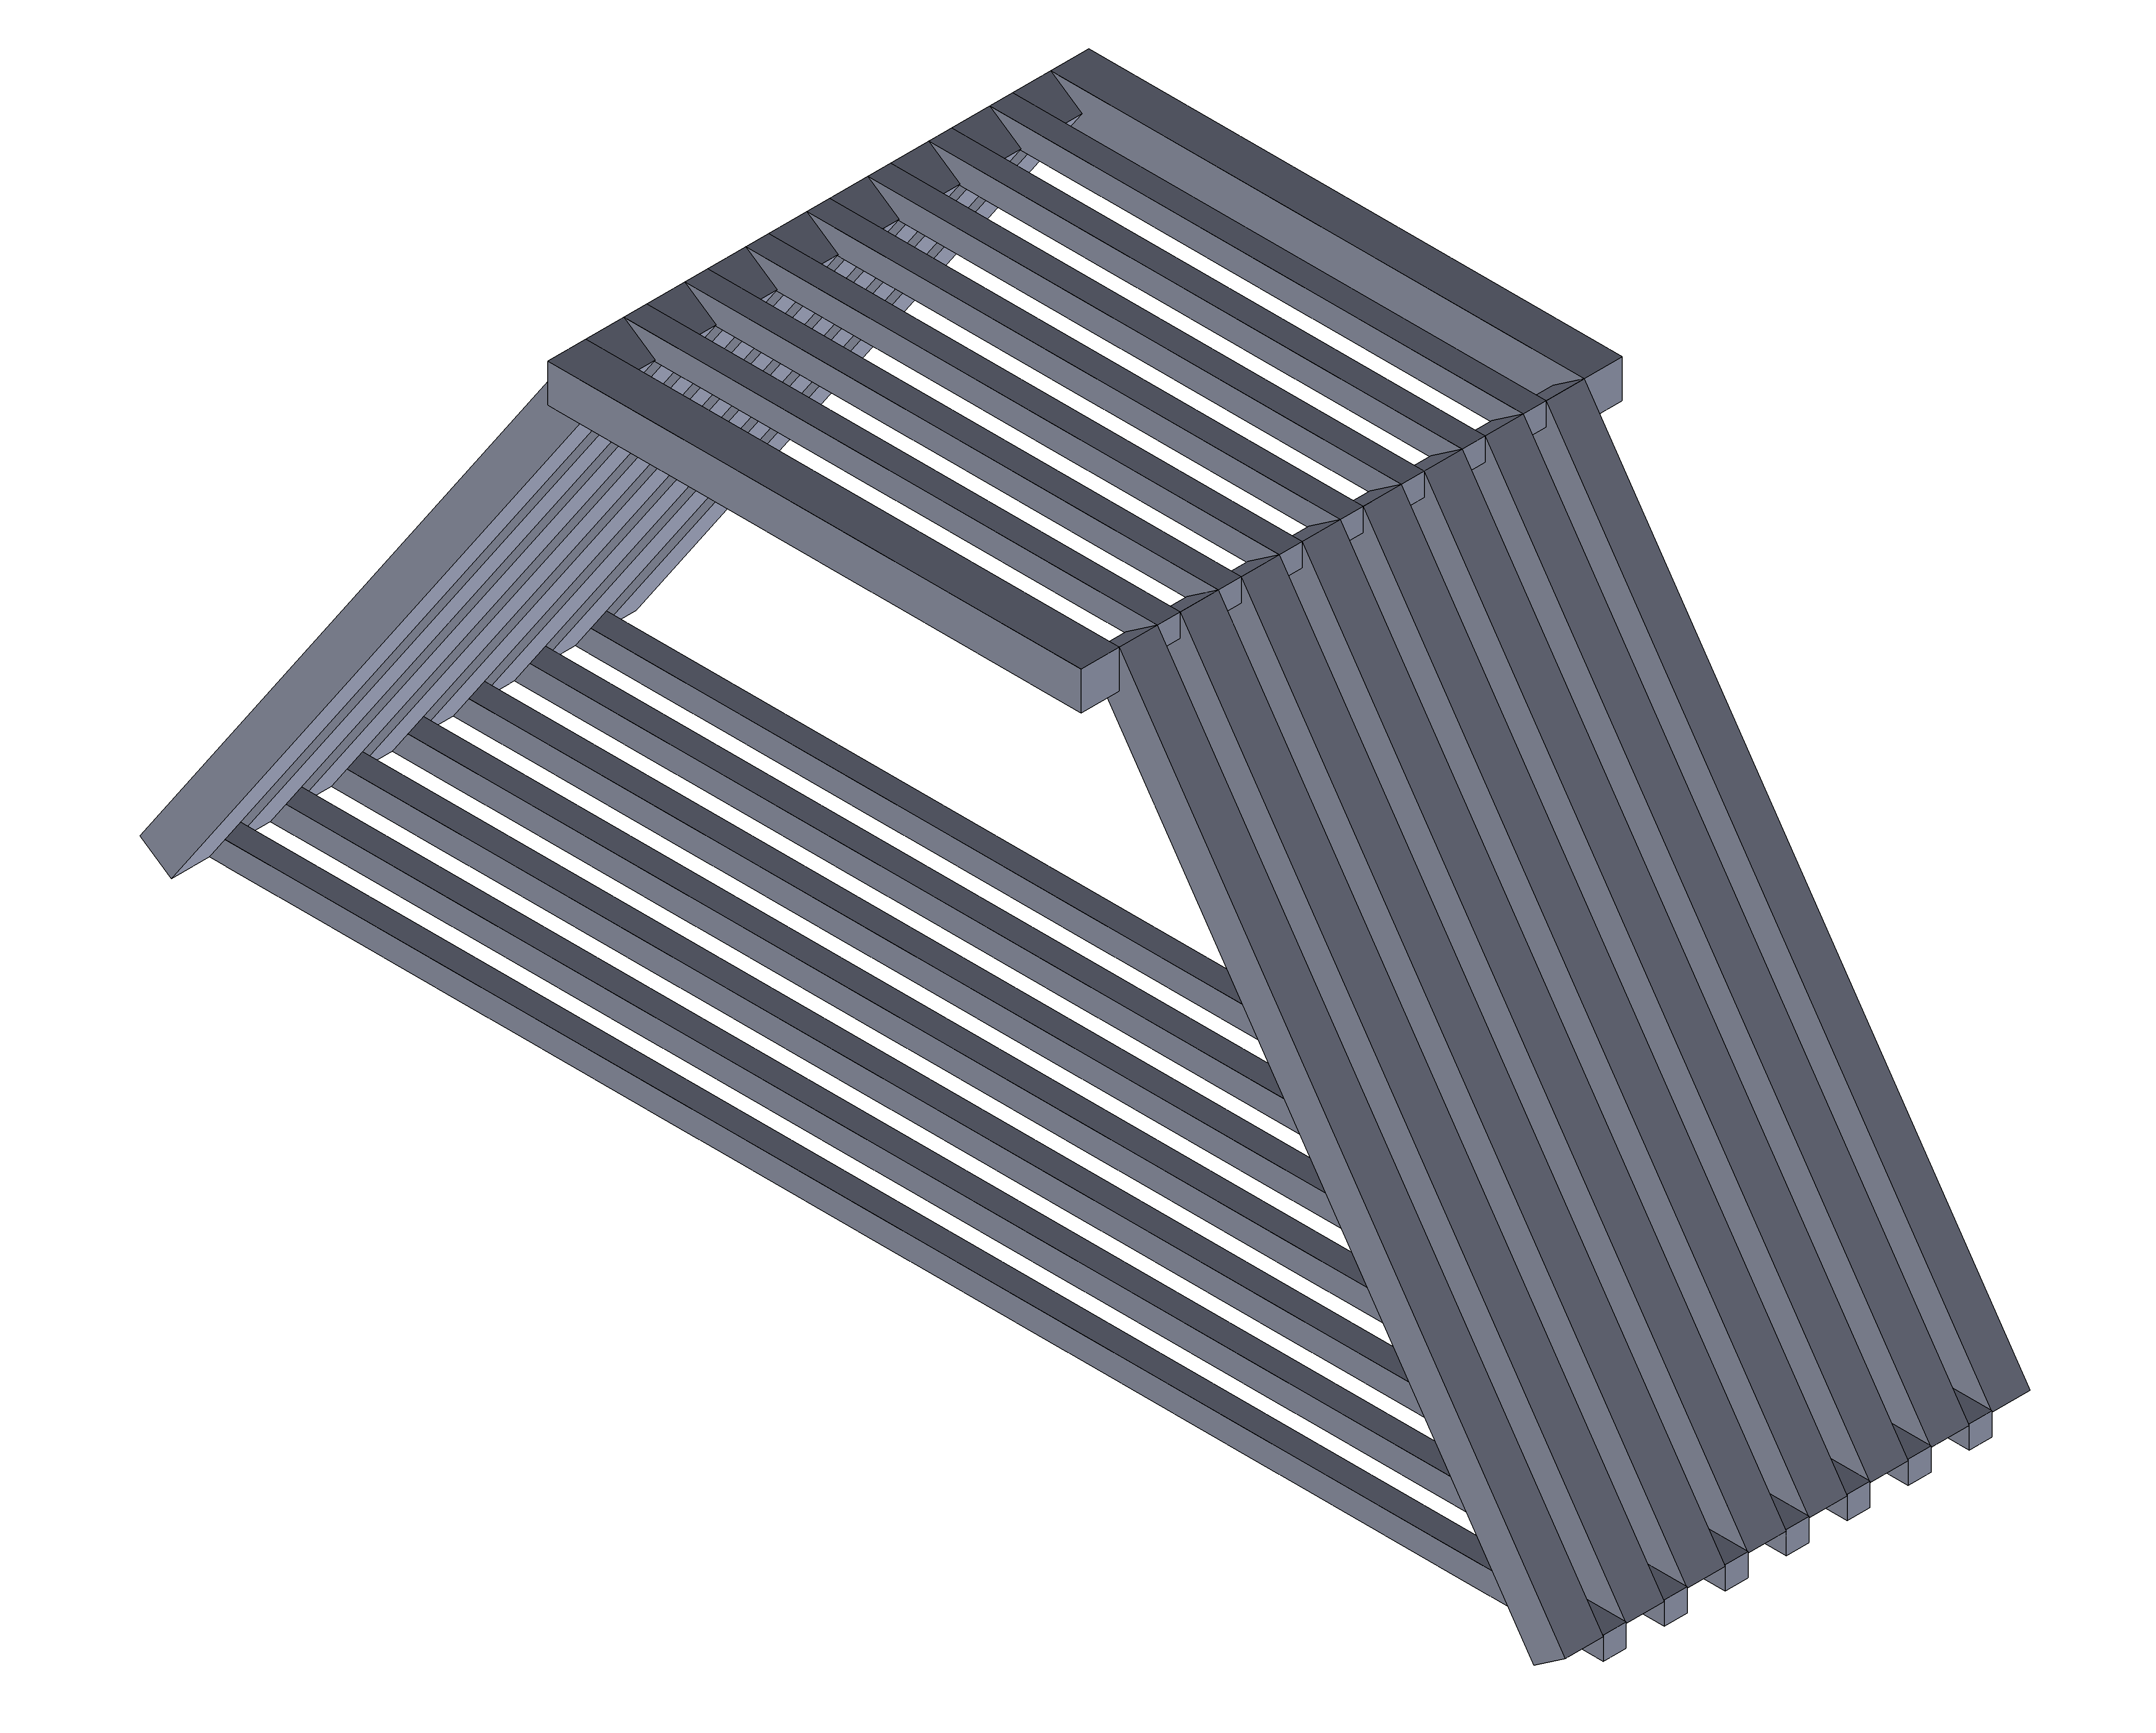
\includegraphics[width=0.5\textwidth]{proj}
			\caption{3D-Projection.}
			\label{proj}
		\end{figure}
		% dimensioned drawing
		\subsection{Methods}
		% construction process 
		% materials Used
		% difficulties faced - measuring accurately, It ended up being 185mm than 187mm and the trapezium was also slightly lopsided by a 1mm, angles are fucked!
		% weight issues - excess glue fail 
		% picture of the materials used
	\section{Analysis}
		Due to the unconventional design, to ease the calculations during the analysis, it was assumed that the load is equally distributed between eight trapezium-shaped trusses. Thus, a single trapezium truss was analyzed, and then extended to approximate the entire bridge. Internal forces, nodes and members are labelled as per Figure~\ref{trap}. As the truss is symmetrical, only two nodes needed to be analyzed.
		\begin{figure}[h!]
			\centering
			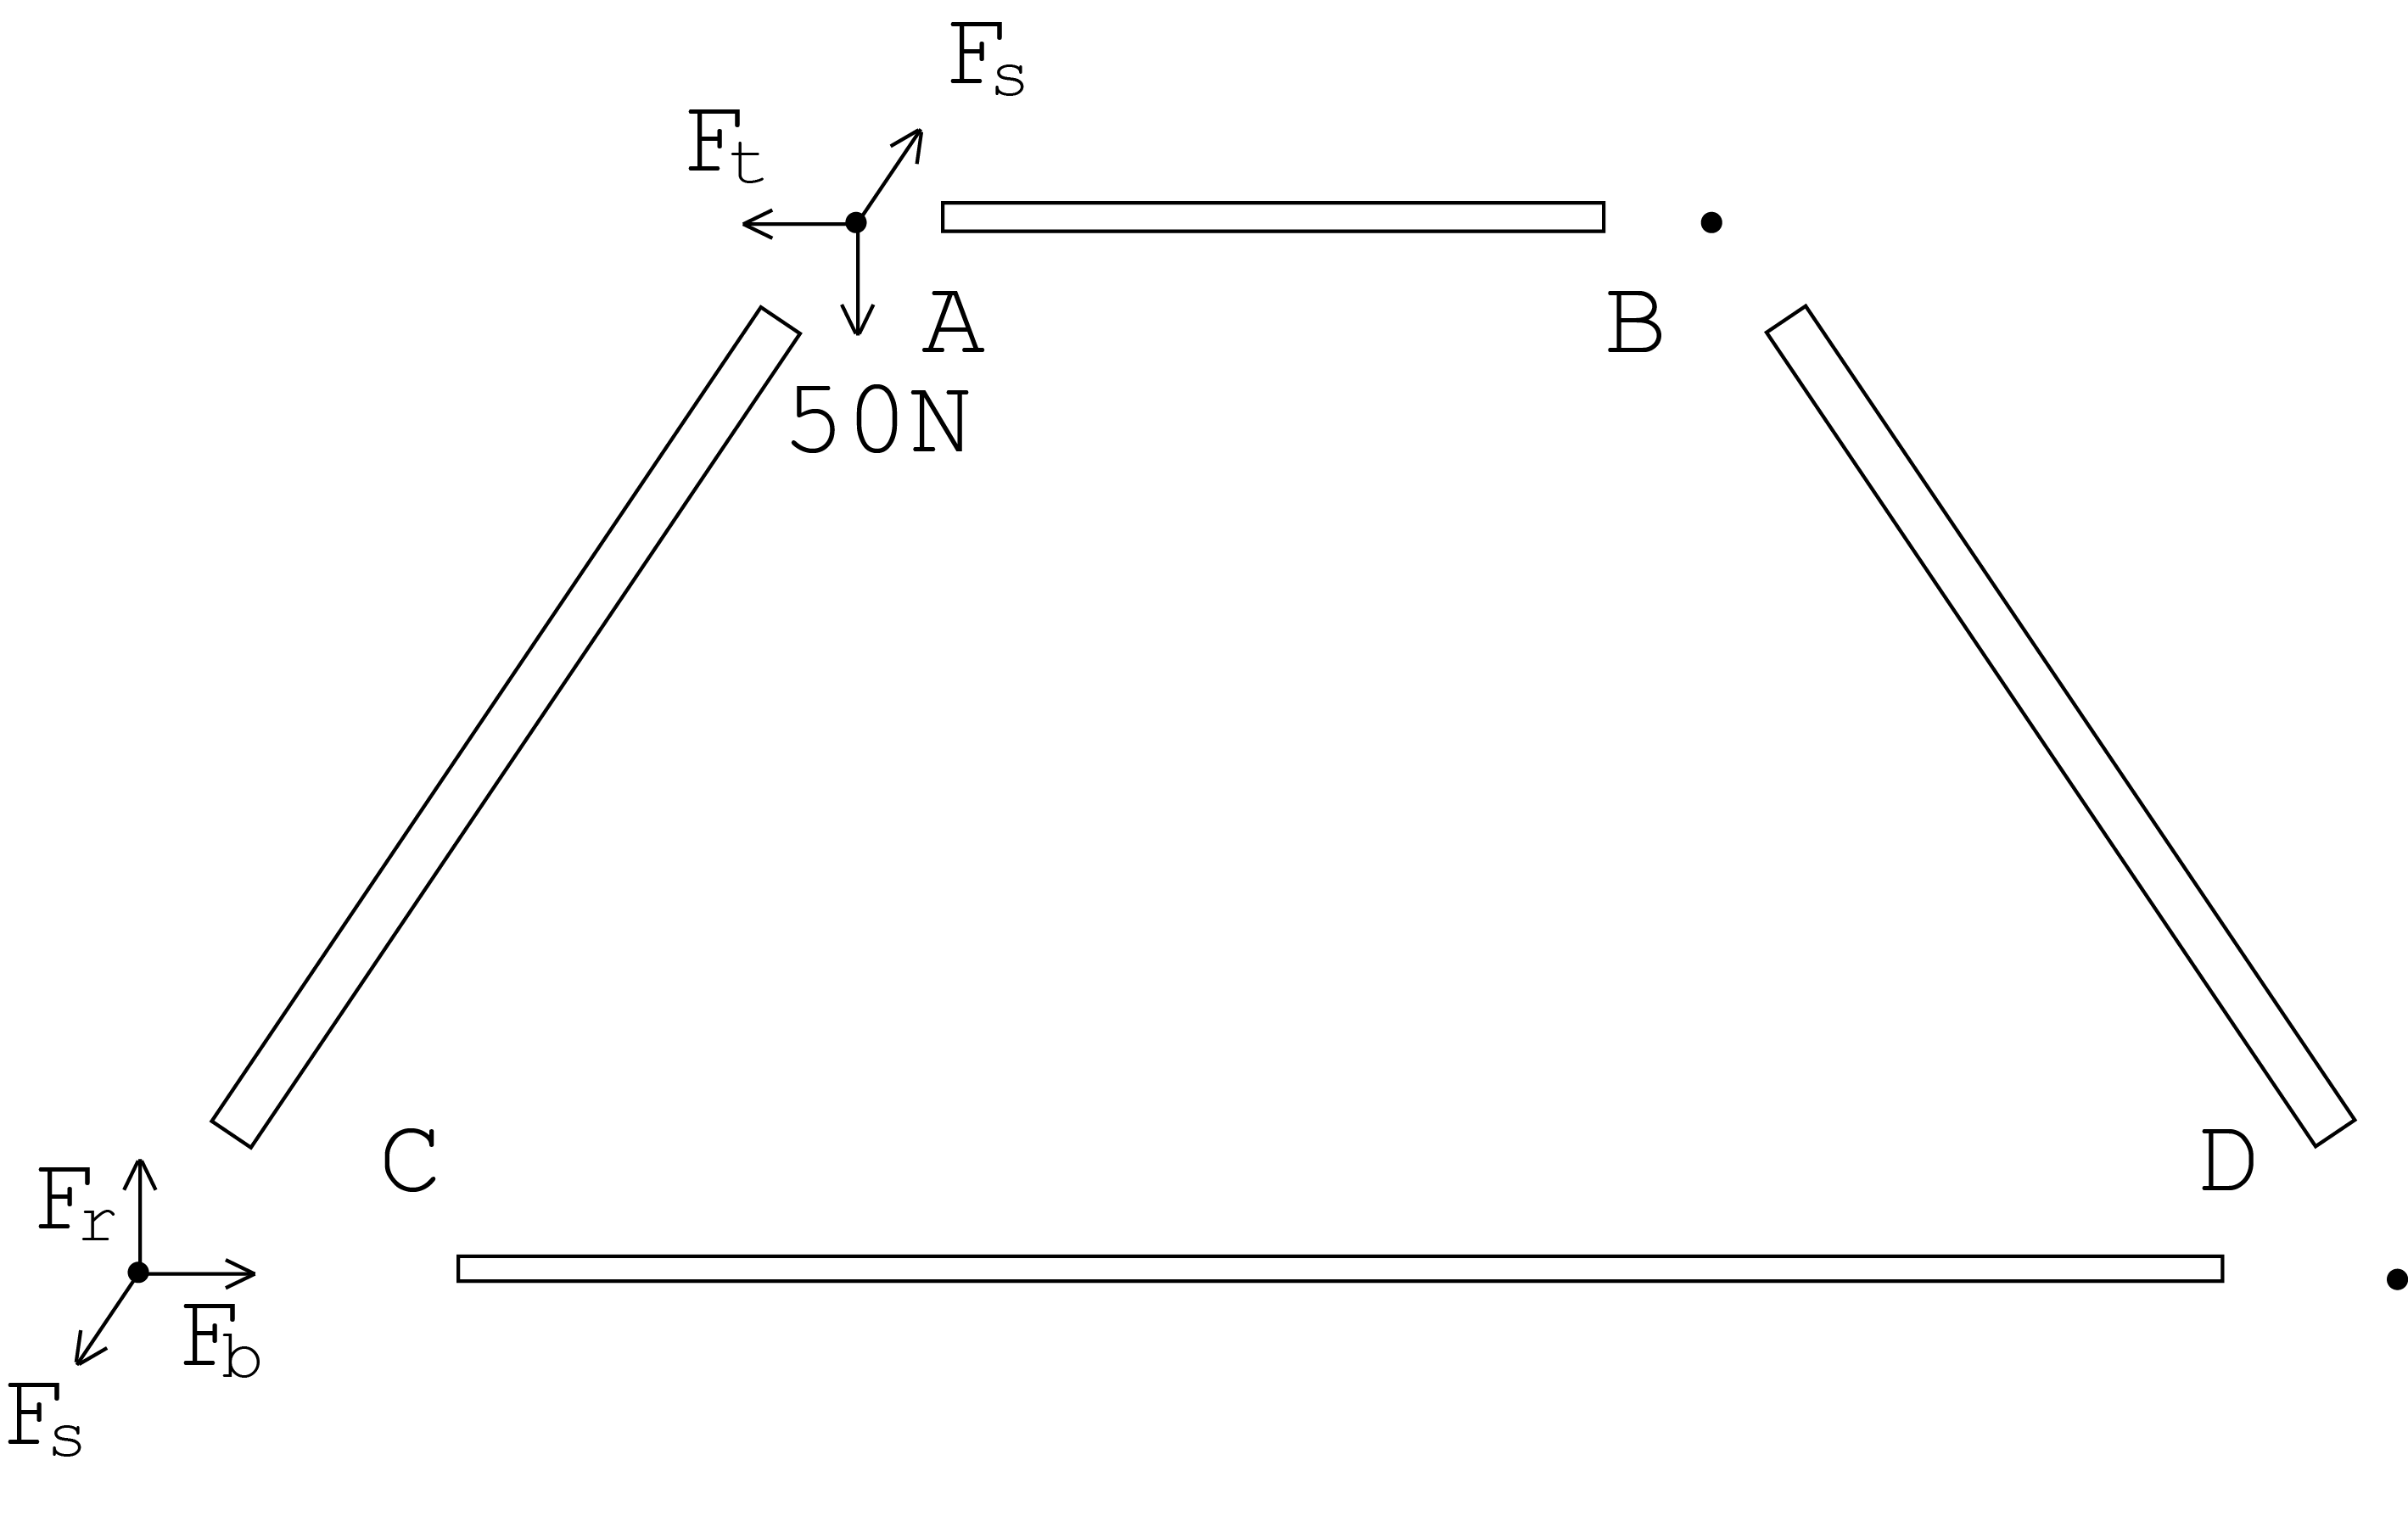
\includegraphics[width=0.7\textwidth]{trapanal}
			\caption{Trapezium truss.}
			\label{trap}
		\end{figure}
		For a load of 100N divided equally between nodes A and B, force equilibrium for nodes A and C are described in equation blocks \ref{eqn1} and \ref{eqn2} respectively.
		% insret calculations here
		\begin{subequations}
			\begin{align}
				F_s \sin 56&=50\mathrm{N}, \\
				F_s \cos 56&=F_t.
			\end{align} \label{eqn1}
		\end{subequations}
		\begin{subequations}
			\begin{align}
				F_s \sin 56&=F_r, \\ 
				F_s \cos 56&=F_b.
			\end{align} \label{eqn2}
		\end{subequations}

		The results of solving the above equations are presented in Table~\ref{loads}. Note that the internal force experienced by members is twice the given value, because it occurs at both ends.
		% table of member loads
		\begin{table}[h!]
			\caption{Member loads.}
			\begin{center}
			\begin{tabular}{ | r | l | }
				\hline
				70 3$\times$3 mm (top) & 33.7 N (c) \\ \hline
				103.75 5$\times$5 mm (side) & 60.3 N (c) \\ \hline
				187 3$\times$3 mm (bottom) & 33.7 N (t) \\ \hline
			\end{tabular}
			\end{center}
			\label{loads}
		\end{table}

		% assumptions
		% max load
		Maximum loads for each member were calculated using the values given in the Assignment sheet. Modulus of elasticity $E=3\mathrm{GN}/\mathrm{m}^2$, standard deviation $\sigma=+2.4/-2.1\mathrm{MN}/\mathrm{m}^2$. Tensile strength $\sigma_t=20\mathrm{GN}/\mathrm{m}^2$,  standard deviation $\sigma=+3.6/-3.4\mathrm{MN}/\mathrm{m}^2$. Compressive strength $\sigma_t=12\mathrm{GN}/\mathrm{m}^2$,  standard deviation $\sigma=+2.1/-2.8\mathrm{MN}/\mathrm{m}^2$. To calculate maximum load from strength values, equation \ref{eqs} was used. The results are presented in Table~\ref{maxloads}.
		\begin{equation}
			\sigma=\frac{P}{A}
			\label{eqs}
		\end{equation}
		\begin{table}[h!]
			\caption{Maximum member loads.}
			\begin{center}
			\begin{tabular}{ | r | l | l | }
				\hline
				& average & $-1\sigma$ \\ \hline
				3$\times$3 mm (c) & 108 N & 82.8 N \\ \hline
				3$\times$3 mm (t) & 180 N & 149.4 N \\ \hline
				5$\times$5 mm (c) & 300 N & 230 N \\ \hline
			\end{tabular}
			\end{center}
			\label{maxloads}
		\end{table}

		Buckling loads were calculated for members under compression (using equation~\ref{eqb}), and it found that the buckling loads of members under compression (see Table~\ref{buck}) did not exceed maximum load, therefore buckling was not critical.
		\begin{equation}
			P_b=\frac{\pi^2 E I}{(kL)^2}
			\label{eqb}
		\end{equation}
		\begin{table}[h!]
			\caption{Maximum buckling loads.}
			\begin{center}
			\begin{tabular}{ | r | l | l | }
				\hline
				& average & $-1\sigma$ \\ \hline
				3$\times$3 70 mm (c) & 163.1 N & 163.0 N \\ \hline
				5$\times$5 103.75 mm (c) & 573.1 N & 572.7 N \\ \hline
			\end{tabular}
			\end{center}
			\label{buck}
		\end{table}
		% reasons

		To predict the maximum load, the weakest section of the bridge had to be found. That was done by first summing up the maximum loads of all top, bottom and side members, (equation block~\ref{eqsa}), using values from Table~\ref{maxloads}, average column.
		\begin{subequations}
			\begin{align}
				P_{top}&=7\times108+2\times300
				&=1356\mathrm{N}\\
				P_{side}&=8\times300
				&=2400\mathrm{N}\\
				P_{bottom}&=7\times180
				&=1260\mathrm{N}
			\end{align}
			\label{eqsa}
		\end{subequations}

		Then the safety rations (defined in equation~\ref{eqr}) were calculated for each section (equation block~\ref{eqrl}), using values from Table~\ref{loads}.
		\begin{equation}
			R=\frac{P_{max}}{P}
			\label{eqr}
		\end{equation}
		\begin{subequations}
			\begin{align}
				R_{top}&=40.2\\
				R_{side}&=39.8\\
				R_{bottom}&=37.4
			\end{align}
			\label{eqrl}
		\end{subequations}

		The lowest safety ratio member will break first, thus bottom was determined to be the breaking point (snapping-type failure). The actual maximum load was determined in equation block~\ref{eqt}, where $P$ is the load used to calculate $R$. The same steps were carried out in equation block~\ref{eqs}, but the strength was assumed to be $1\sigma$ below average.
		\begin{subequations}
			\begin{align}
				F&=\frac{R P}{2} \\
				&=1869.4
			\end{align}
			\label{eqt}
		\end{subequations}
		\begin{subequations}
			\begin{align}
				F&=\frac{R_{\sigma} P_{\sigma}}{2} \\
				&=1551.6
			\end{align}
			\label{eqs}
		\end{subequations}

		The average of the two $1710.5\mathrm{N}$, was chosen as predicted maximum load.
	\section{Results}
The predicted strength of the bridge was 1700N while the maximum force that it sustained during the test was 875N. This the most significant contributor to this imprecise prediction was that the bridge was too short to comfortably span the 18cm gap. Furthermore, gluing techniques were not researched and as a result the joints were not as strong as they otherwise may have been.

Originally the bridge was designed to be 18.7cm long – just enough to span the 18cm gap. However, on the day of testing the bridge was found to be over the weight limit and in an attempt to fix this the bridge was sanded. After the sanding process the bridge was found to be 18.4cm, which left 2mm either side of the gap. Consequently, during the test the bridge slipped under the applied force and rotated so that roughly half the length of one side of the bridge was no longer in contact with the wood block. As a result the proportion of the distributed load applied to this section of the bridge produced a shear at this point in the row of joints. This shear force was maximum at point A (shown in Figure~\ref{loadtop}). This caused the joint at this point to break which can be seen in Figure~\ref{failtop} as the middle joint – the fifth joint from the top.
		\begin{figure}[h!]
			\centering
			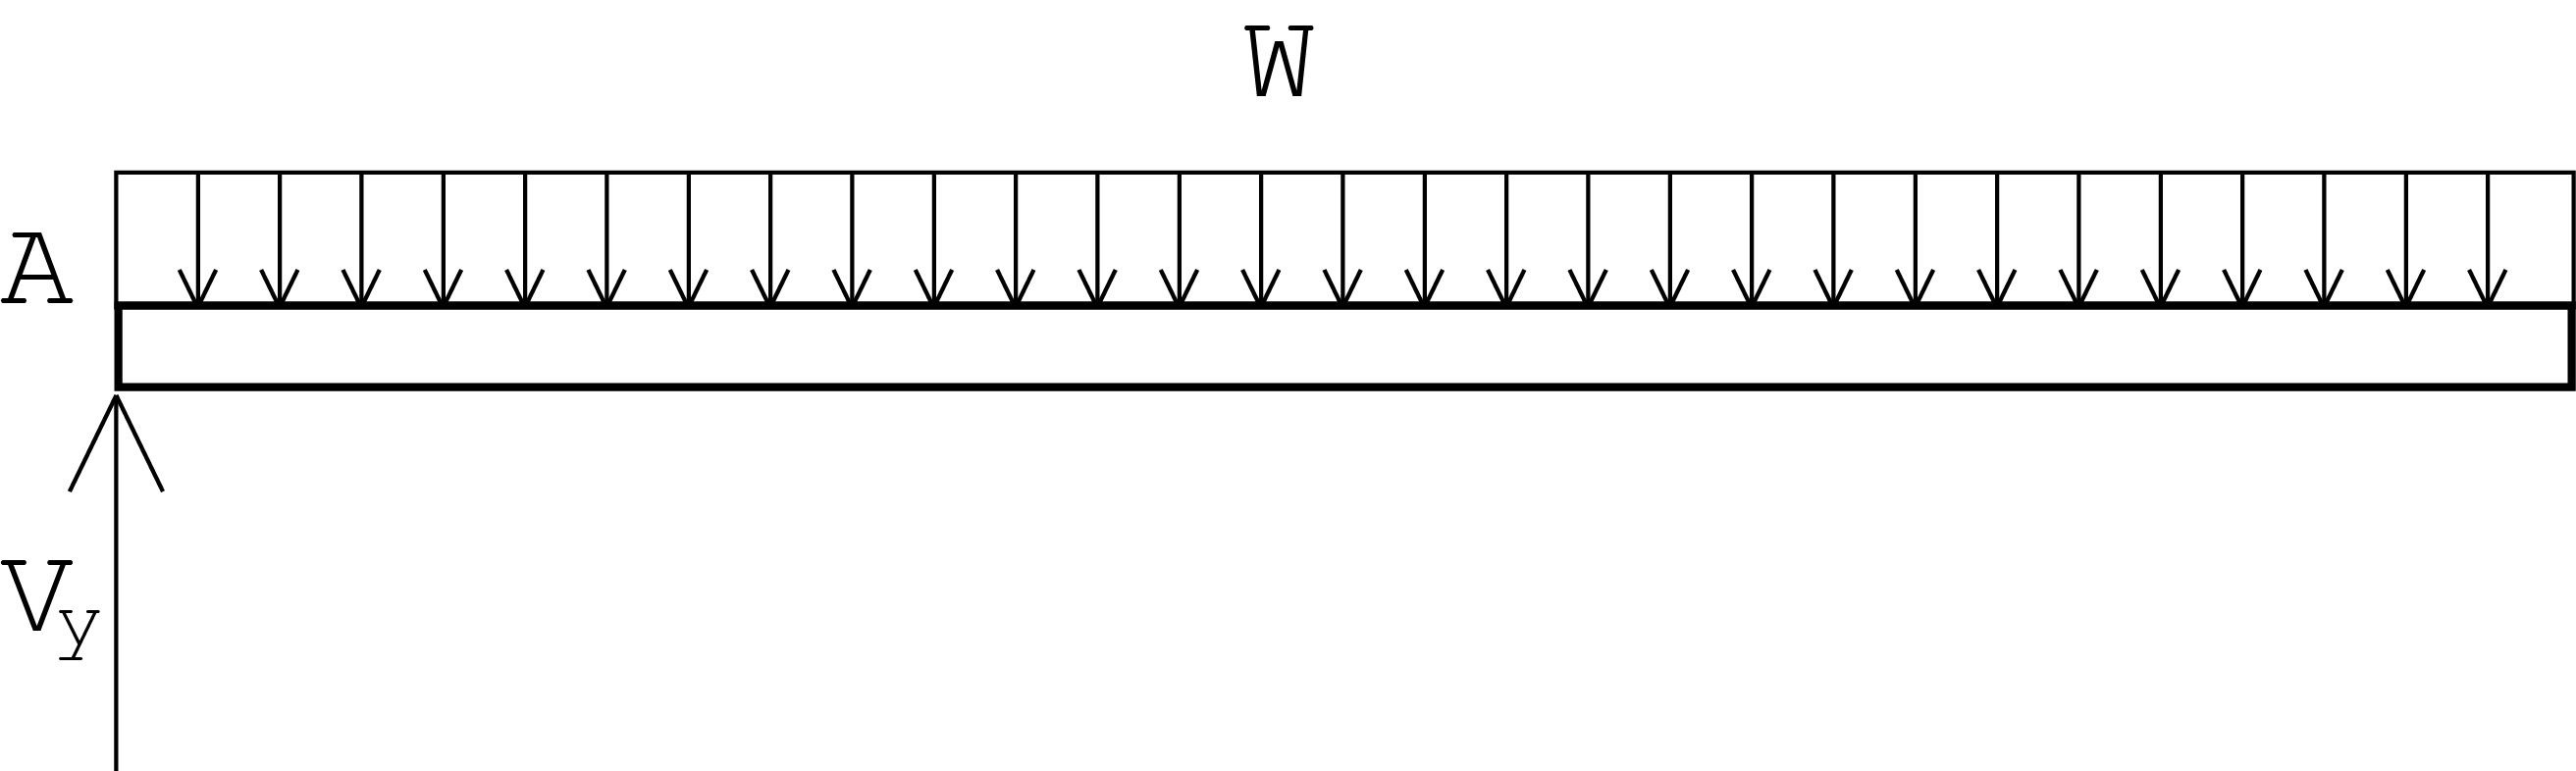
\includegraphics[width=0.7\textwidth]{loadtop}
			\caption{Half of the top joint row under load.}
			\label{loadtop}
		\end{figure}

If the vertical force system acting on the top member where the load is applied is taken then this process can be better examined. The pressure exerted by the loading plate is assumed to be resolved into distributed loadings along the joints at either end of the 7$\times$7cm area at the top of the bridge. For this analysis the line of joins is taken as a rigid body with a fixed support reaction at A where it joins the joints that are part of the bridge that has not come off the block. Halfway along the length of this rigid body the resultant force is positioned as per figure (shown in Figure~\ref{loadtop}).  For equilibrium the hypothetical support reactions at A must be equal and opposite to the resultant force and moment. If the structure had not slipped, the vertical forces in the side pieces of the structure would cancel out this distributed load but due to the slipping they do not. As the side of the bridge was pushed downwards, the side members in the bridge would have applied some force to the upper row of joints as the structure tried to maintain its integrity creating another distributed load. This loading however would be small in comparison to the applied load of the block and is thus left out in the following analysis.

Now the internal forces in this rigid body can be analysed using the distributed load and the support reactions.  Figure~\ref{loadtop} shows the distributed load $w \mathrm{(N/m)}$ on the unsupported segment and hypothetical support reaction $A_y$ under an arbitrary load. The intensity of the distributed load is given by the total loading applied by the loading plate divided by $0.14\mathrm{m}$, the combined lengths of the two lines of joints. The equation for the internal shear force along the line of joints is: $V=A_y–wx$ where $x$ is the distance from point $A$ and $V$ is the internal shear force. This equation shows that the internal shear force is maximum at point $A$ ($x=0$) which is where the break occurred. The equation for the internal moment is $M = A_yx –0.5(wx^2)$, where $M$ is the internal moment. $M$ is maximum at $x = 0.035$ or the furthest point along the body from $A$. In reality the moment may be reduced slightly as the structure may bend to compensate for the applied load.

After the joint at point $A$ snapped, the unsupported side of the bridge was displaced downwards, creating a moment about the other row of joints. Initially this caused the fourth joint from the top on the right (as per Figure~\ref{failtop}) to split. Then the joints below it also began to split. As the applied force increased so did the moment and consequently the splitting of the joints.
		\begin{figure}[h!]
			\centering
			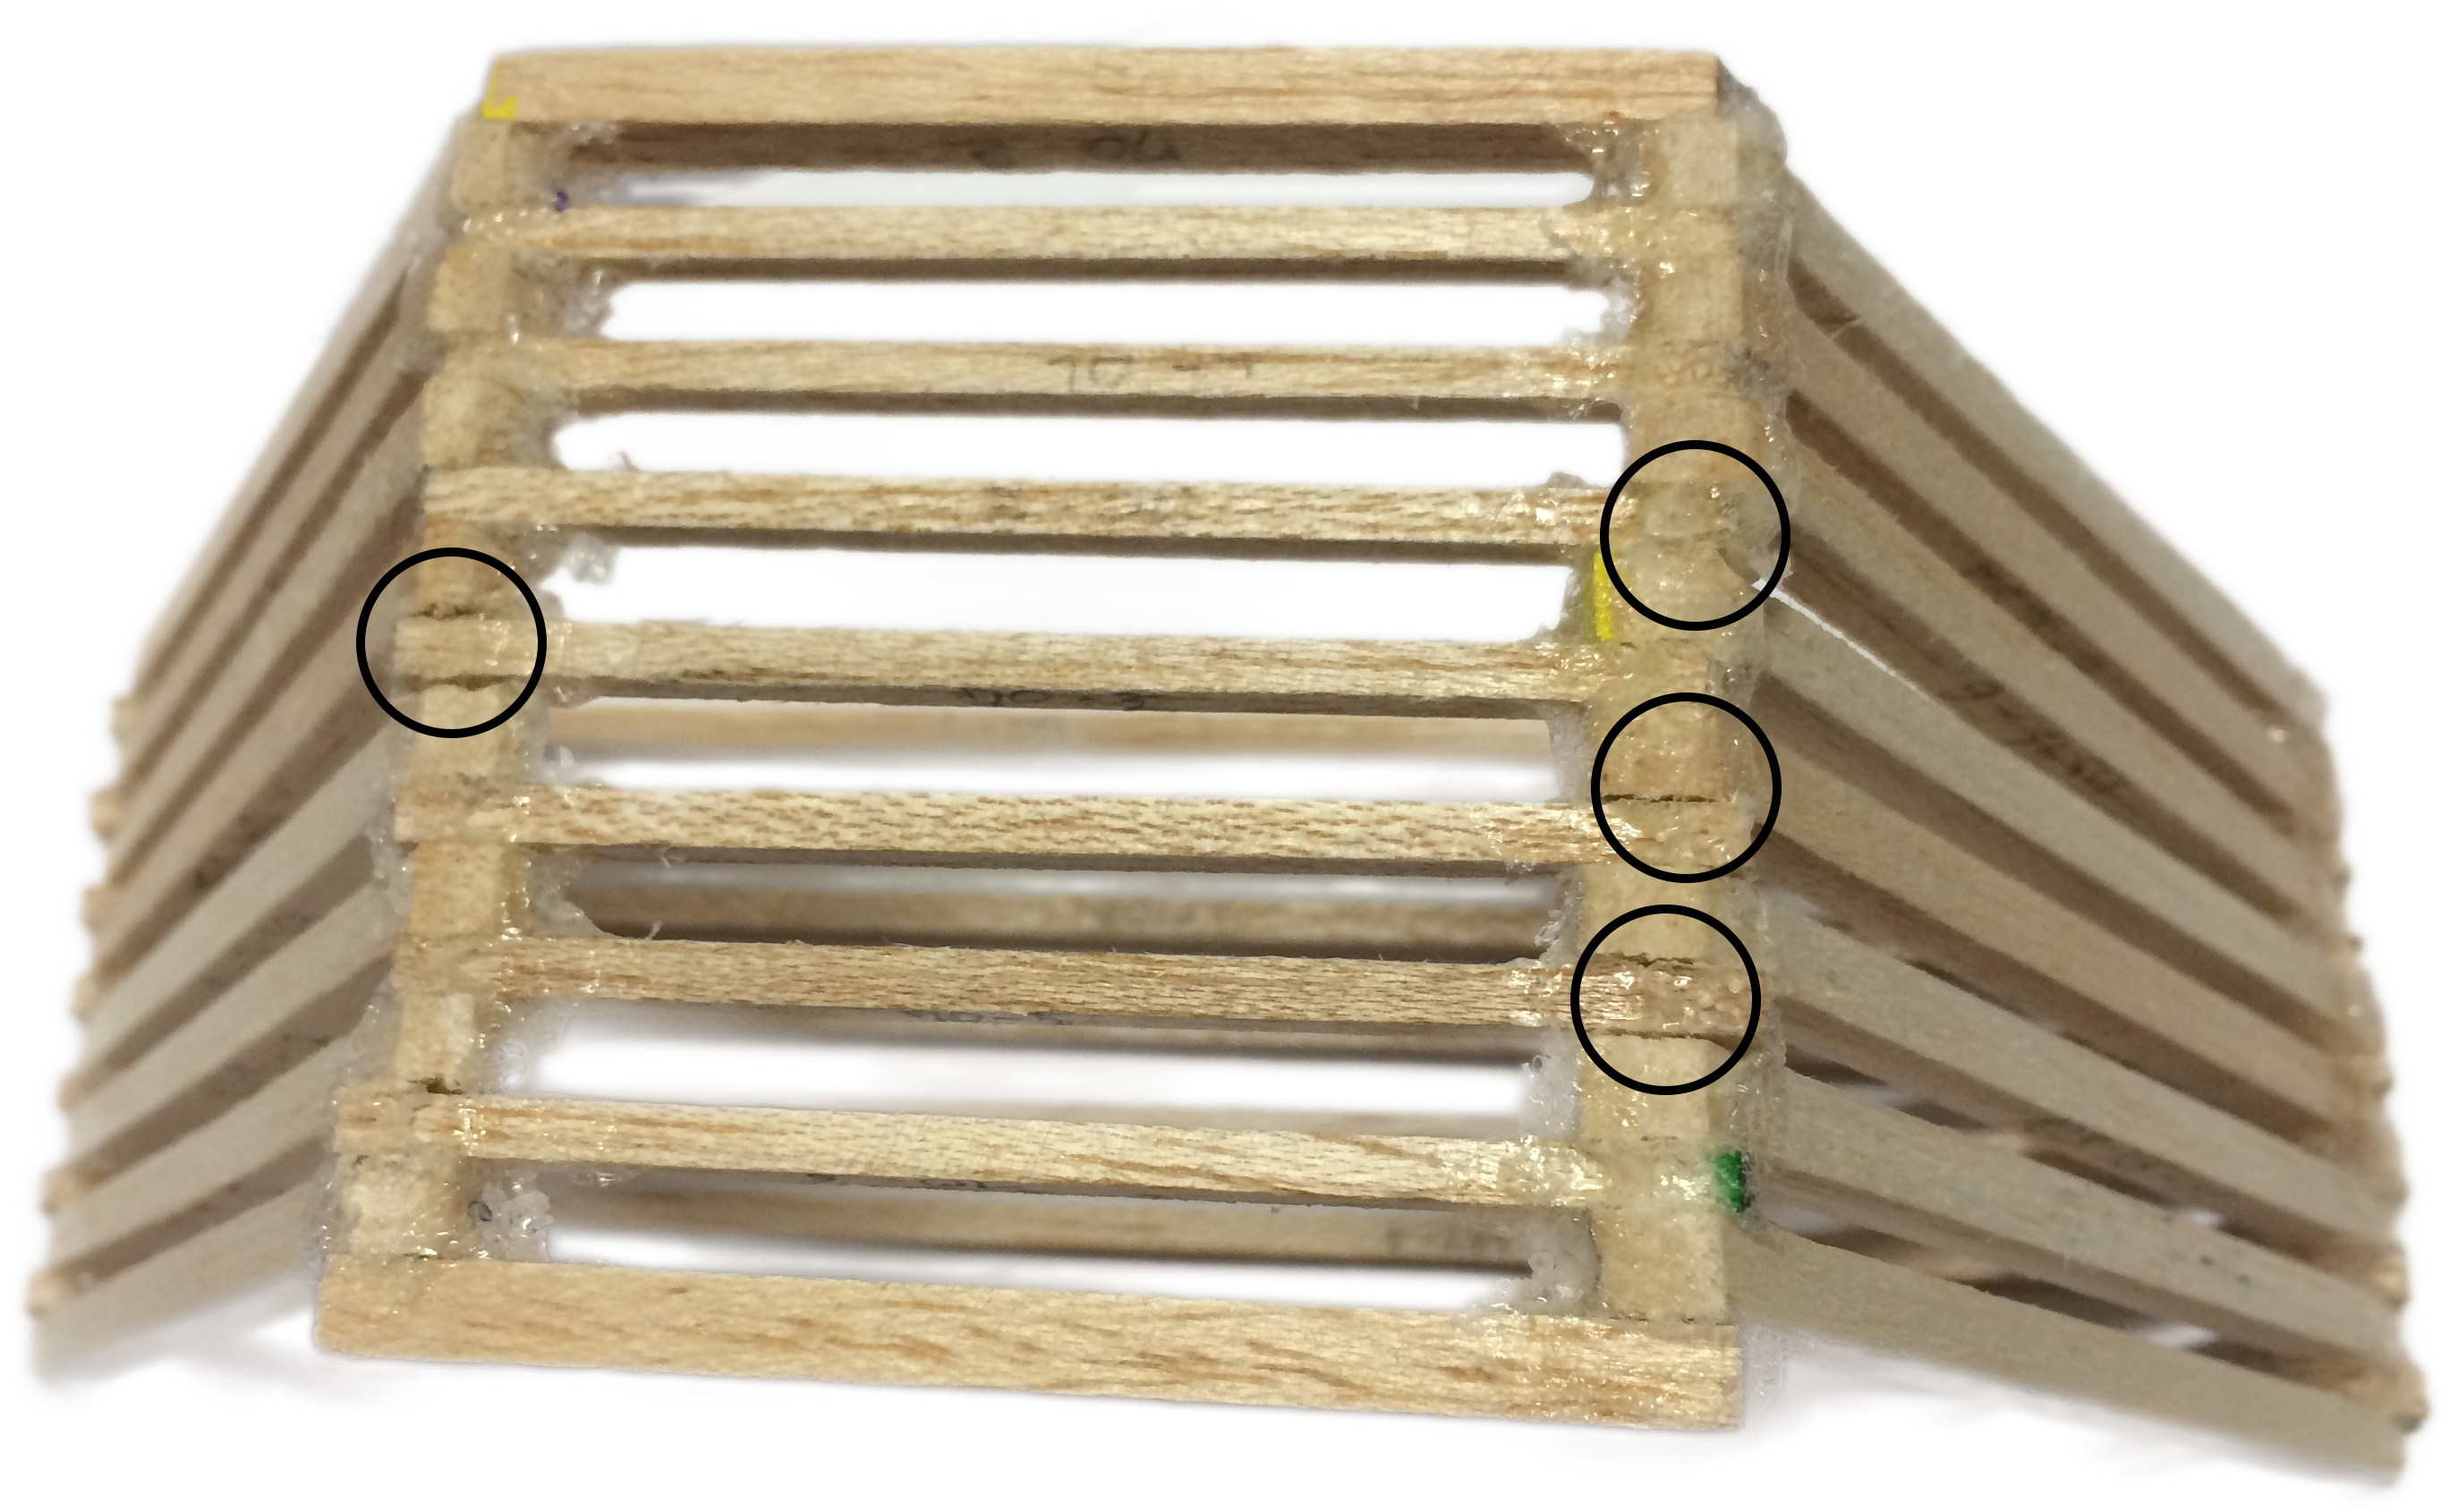
\includegraphics[width=0.5\textwidth]{failtop}
			\caption{Top of the bridge.}
			\label{failtop}
		\end{figure}

After these joints snapped half of the bridge was incapable of bearing load and as a result the load bearing capacity of the bridge was halved. This is reflected by the quotient of the measured maximum load and the predicted maximum load, which is approximately one half. So had the bridge been longer and thus protected from slipping, it is likely that it could have supported the maximum predicted load.

When the forces bridge slipped, the joints showed little resistance and failed a within a second after. The reason for this was that far too much glue was used on the joints. According to (reference), the strength of a joint glued with balsa cement is inversely proportional to the distance between the two surfaces until the distance reaches the width of the molecules of the glue. While several drops of glue were applied to each joint in this bridge (reference) states that even one drop of glue is excessive. In applying such an excessive amount of glue the joints were significantly weakened as the distance between the surfaces of the balsa pieces was increased. However, a glued joint can only be as strong as the material being held together and balsa wood is weaker when a force is applied perpendicular to its grain orientation. The application of significant shear force between joints would cause the wood itself to break and split off. As demonstrated in the analysis above, the maximum shear force in the row of joints is equal in magnitude to the resultant force of the applied load, ignoring the contribution of the distributed load from the side members. Even if it were taken into consideration, the shear force is too high for a joint to tolerate.

If the correct gluing method was applied to the joints of the bridge its maximum loading may have been increased slightly but the primary cause of failure was the length of the bridge and the resultant slipping.
%What was the final load it could hold?

	\bibliography{bib}
\end{document}

